% cone20-simple.tex

\section{Microscale combustion}
\label{micro-combustion}
%
Here is an example of a reacting flow at submillimeter scale. The gas mixture of
stoichiometric methane/air is fed to a 2-D micro-channel at the dimension of 5 mm
(in length) $\times$ 0.3 mm (in height). The reaction mechanism of 19-species and
84-reaction methane/air chemistry (DRM19)~\cite{DRM19} is used in the simulation.
The method of ``IgnitionZone'' is switched on for the initial 1 ms in order to
trigger the combustion and then switched off subsequently. Figure~\ref{fig:micro-combustion-domain}
shows the computational domain.

\begin{figure}[h]
\begin{center}
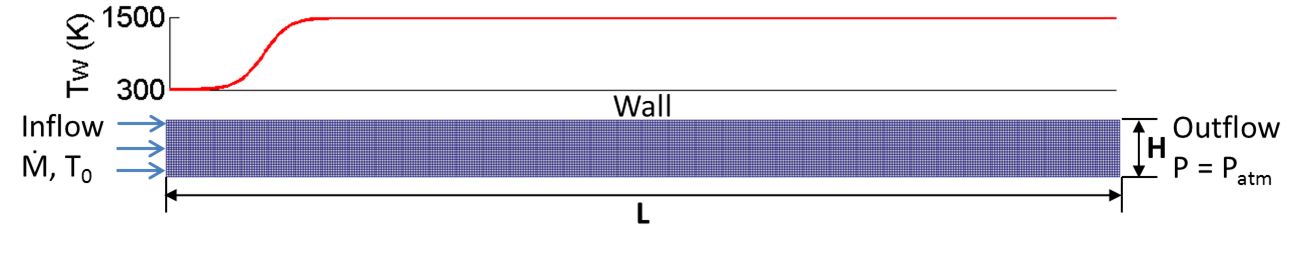
\includegraphics[width=15cm]{../2D/micro-combustion/computational_domain.png}
\caption{Computational domain of the planar micro-channel and boundary conditions used.}
\label{fig:micro-combustion-domain}
\end{center}
\end{figure}

\subsection{Input script (.py)}
%
\noindent\topbar
\lstinputlisting[language={}]{../2D/micro-combustion/microchannel.py}
\bottombar

\subsection{UDF Boundary conditions}
%
At the inlet of the channel, an inflow boundary condition based on the characteristic
wave relations~\cite{Poi_JCP_1992} is employed. It is capable of absorbing acoustic waves
due to the chemical heat release and heat exchange between the flow and the wall. 
The gas total temperature ($T_0$), mass flow rate ($\dot{M}$) and incoming species
mass fractions are specified.\\
\noindent\topbar
\lstinputlisting[language={}]{../2D/micro-combustion/udf-massflux-in.lua}
\bottombar

At the wall of the channel, a hyperbolic tangent temperature profile is prescribed.
The temperature ramps from 300 K to 1500 K over the initial 1 mm of the channel length
and maintains at 1500K for the rest length of the combustor.\\
\noindent\topbar
\lstinputlisting[language={}]{../2D/micro-combustion/udf-wall.lua}
\bottombar

\subsection{Running the simulation}
%
This simulation is running on Barrine cluster (the High-Performance Computing Unit at UQ)
using 64 processors, with a shell script:\\
\noindent\topbar
\lstinputlisting[language={}]{../2D/micro-combustion/queue.sh}
\bottombar

This heavy task will take approximately 10 days wall clock time to reach a stable solution.

\subsection{Results}
%
Figure~\ref{fig:CH3} plots the temporal evolution of CH$_3$ radicals which are responsible
for the establishment of the flame front. In the initial 0.1 ms, CH$_3$ radicals are generated
and accumulated near the walls. Then the flame is established and bifurcated into two branches:
The main flame propagates upstream and finally gets stablized, while the bifurcated flame propagtes
downstream and then flows out of the domain. After around 4 ms, a stable solution is obtained.

\begin{figure}[h]
\begin{center}
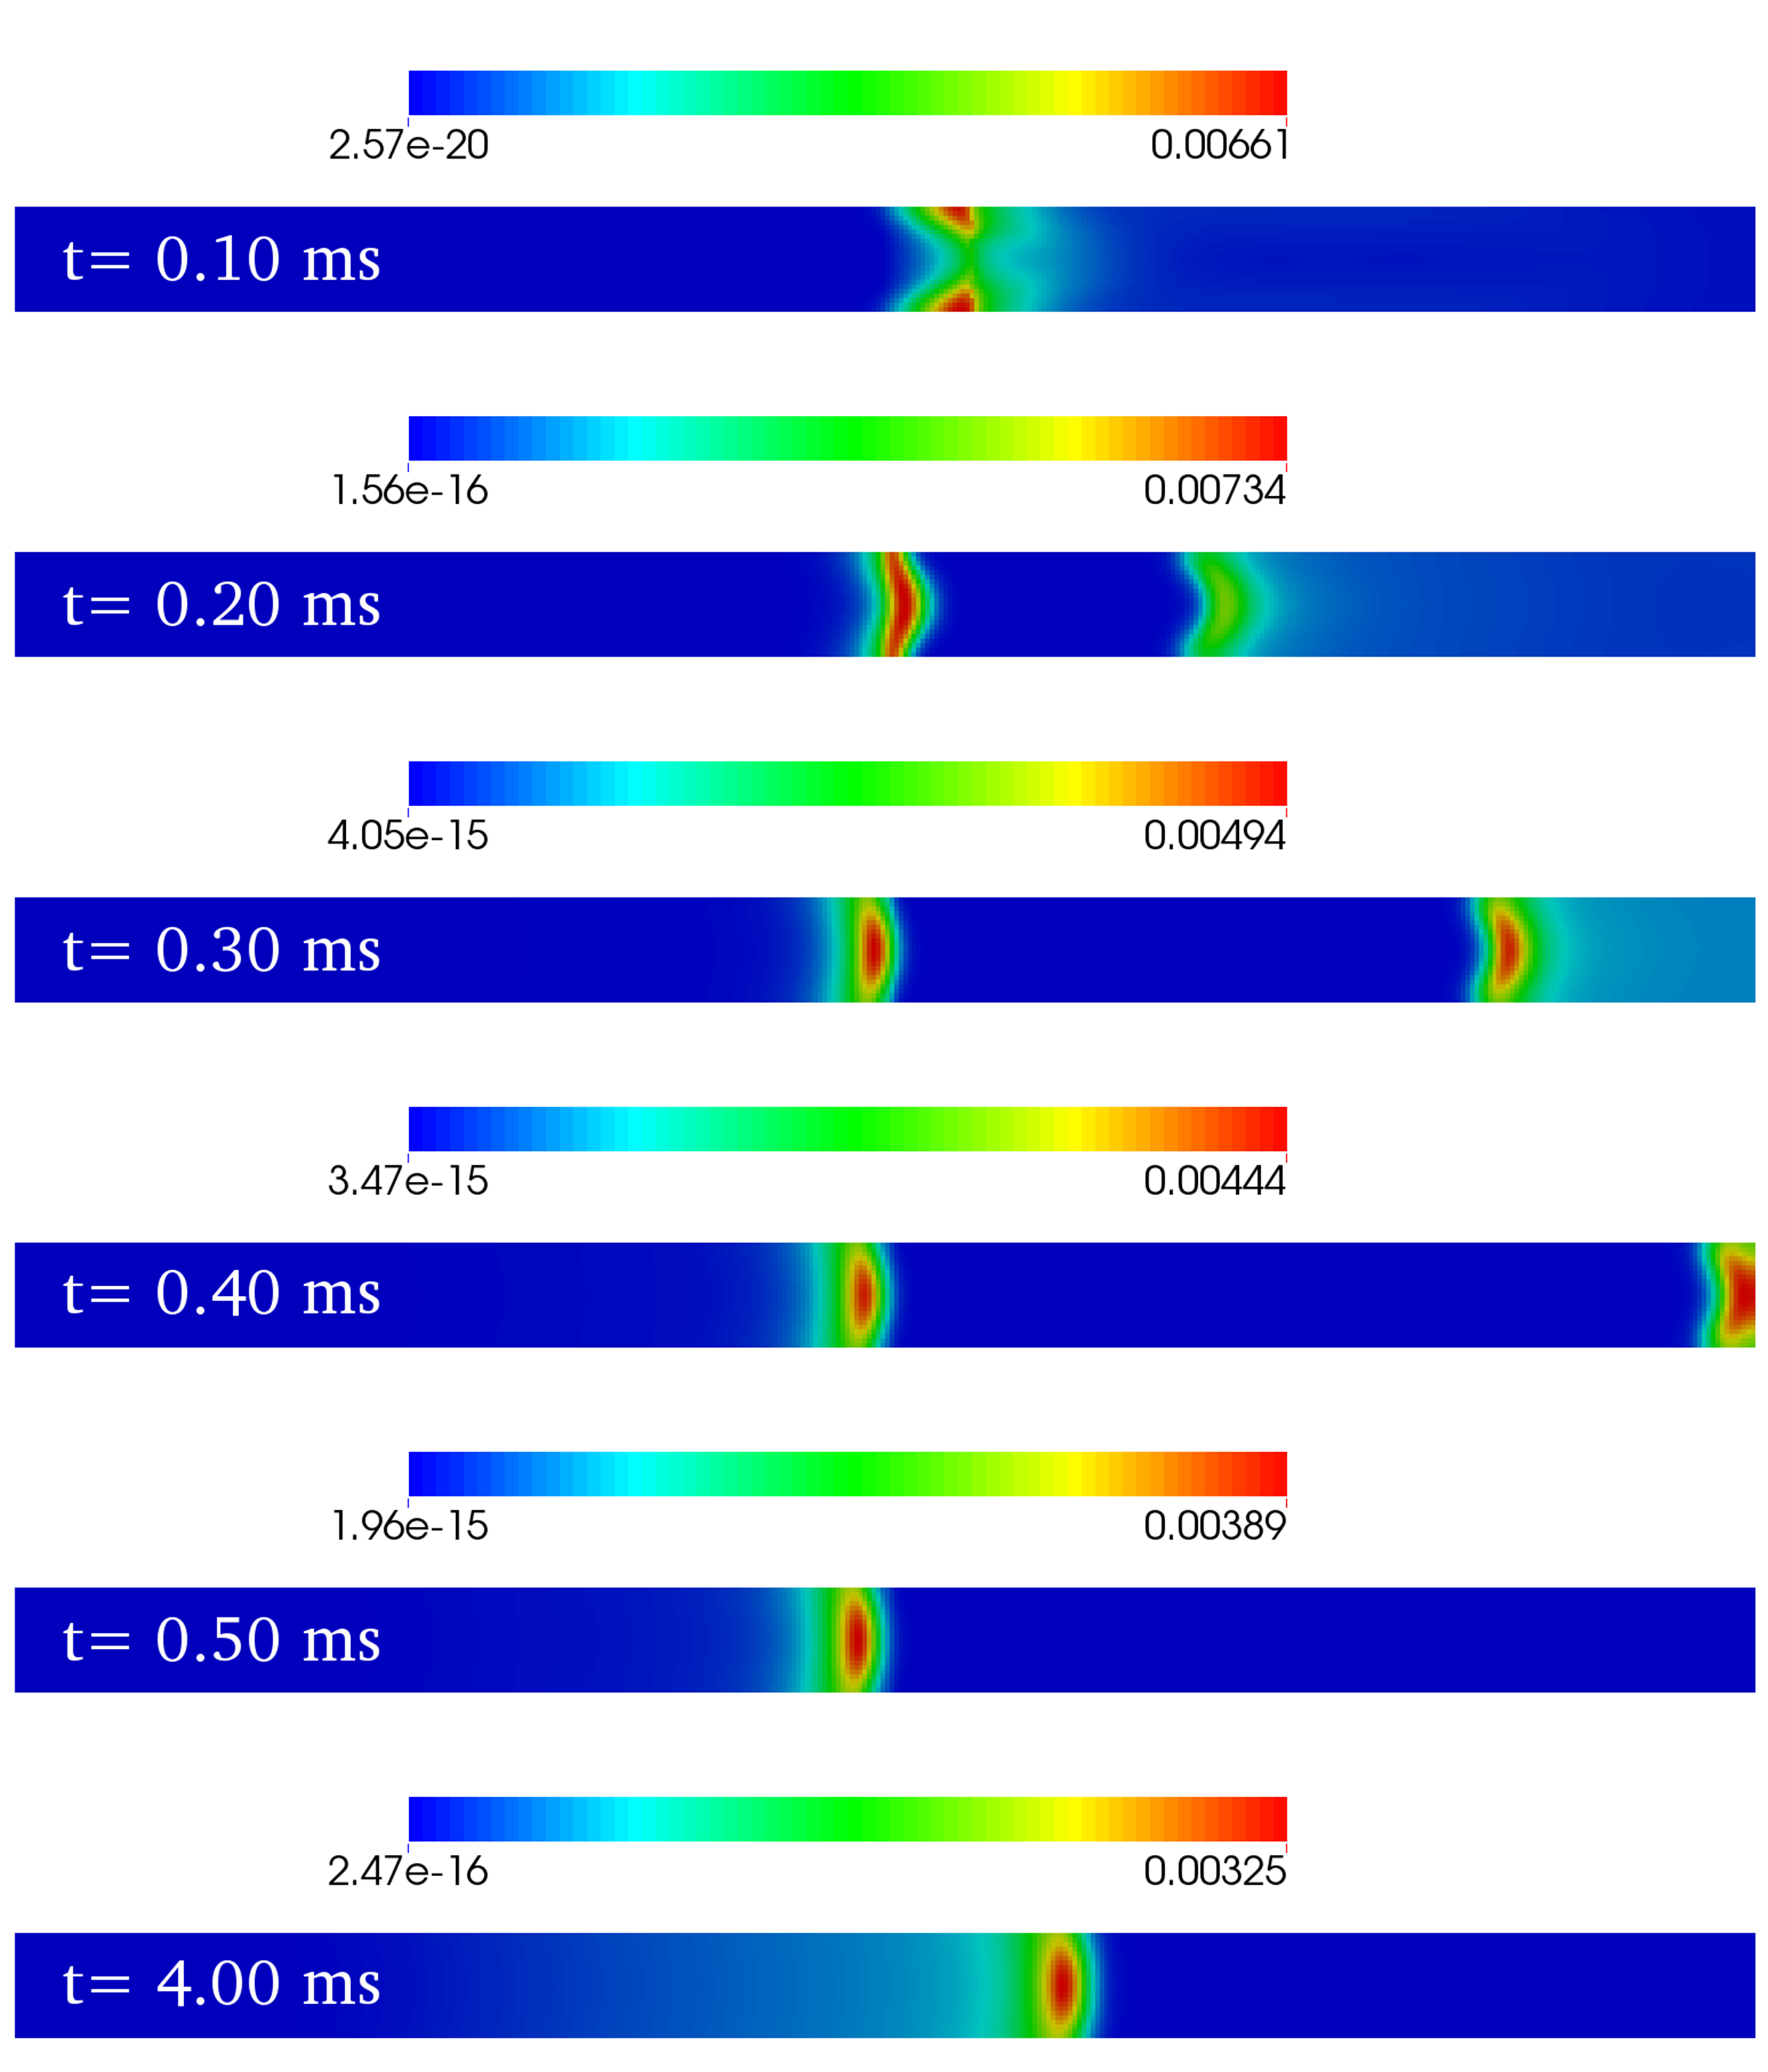
\includegraphics[width=15cm]{../2D/micro-combustion/CH3.png}
\caption{Temporal evolution of CH$_3$ radical concentrations.}
\label{fig:CH3}
\end{center}
\end{figure}